\chapter{Resultados}

\section{Modelo de simulação fluidodinâmica computacional}


No contexto de um fluxo específico, a ocorrência de dano erosivo é observada em várias áreas das paredes da tubulação, devido às colisões de cascalhos em várias regiões durante o escoamento, sob diferentes condições. Contudo, embora existam diferentes magnitudes de taxa erosiva, numa mesma condição de fluxo e para um mesmo material, o que de fato interessa para a análise de risco, é o ponto da tubulação onde ocorre a maior taxa erosiva, ou seja, a região onde o material irá falhar primeiro. Deste modo, a taxa erosiva máxima é a função-objetivo de análise deste trabalho em todos os cenários de simulação de fluxo estacionários realizados. Conforme demonstrado na Figura \ref{fig:maiorerosao}, para este exemplo de simulação fluidodinâmica, o valor máximo de erosão foi de aproximadamente 8E-08 kg/m.s² ocorrendo num ângulo de aproximadamente 70° da curva. 

\begin{figure}[H] 
    \centering  
    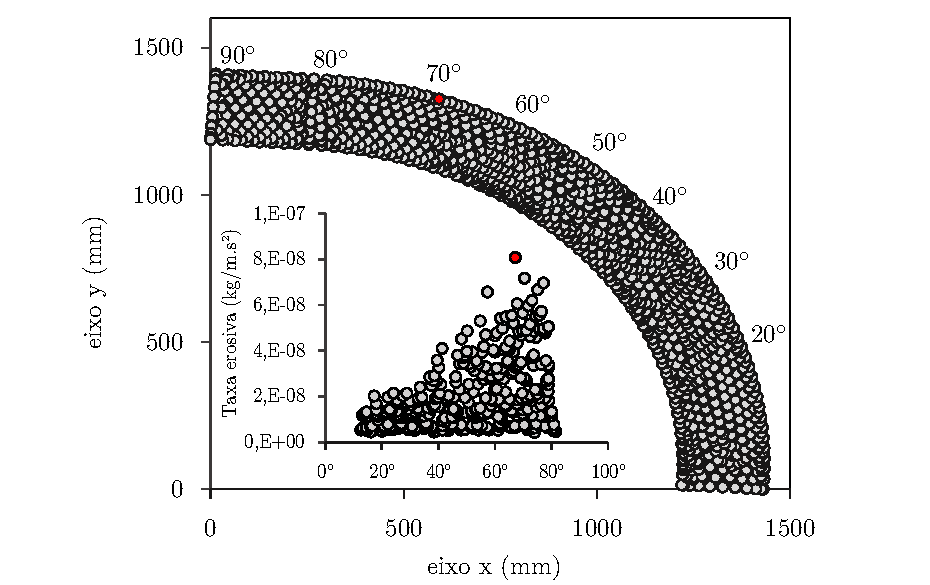
\includegraphics[width=0.85\textwidth]{Figuras/pontodemaiiorerosao.pdf}  
    \caption{Ponto de maior erosão resultante da simulação fluidodinâmica computacional.}  
    \legend{Fonte: o autor.}
    \label{fig:maiorerosao}  
\end{figure}

O modelo de \citeonline{oka} aplicado em simulações computacionais CFD, foi comparado e validado com base em ensaios experimentais em curvas de 90º de raio curto \cite{liuuh}, a mesma geometria utilizada no presente trabalho (Figura \ref{fig:cfdgeometria}). Portanto, as taxas de erosão foram obtidas utilizando o modelo proposto por \citeonline{oka} matematicamente formulado na Equação \ref{equationoka}. Este modelo foi relacionado interativamente com as equações de transporte do fluido e das partículas, de modo que ao final fosse possível obter as taxas de erosão ao longo de toda parede do duto.

A convergência do modelo fluidodinâmico foi analisada verificando os resíduos das equações governantes do modelo (Figura \ref{fig:cfdcontinuidade}). Embora haja baixos valores residuais e um comportamento de convergência das equações governantes, é possível que a solução física de escoamento não convirja. Desse modo, como alternativa complementar para análise do modelo, foi monitorado a convergência física do parâmetro de velocidade de escoamento na saída do fluido do sistema (Figura \ref{fig:cfdcontinuidade2}).

\begin{figure}[H] 
    \centering  
    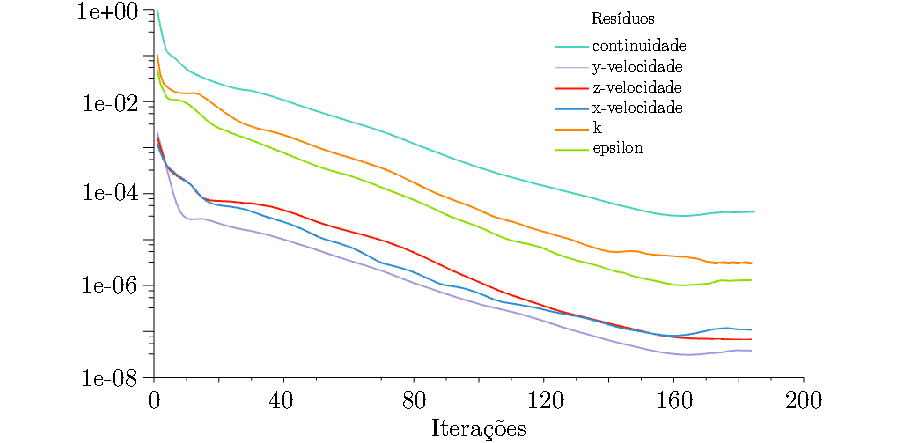
\includegraphics[width=0.90\textwidth]{Figuras/cfddecontinuidade.pdf}  
    \caption{Convergência dos resíduos do modelo fluidodinâmico.}  
    \legend{Fonte: o autor.}
    \label{fig:cfdcontinuidade}  
\end{figure}


\begin{figure}[H] 
    \centering  
    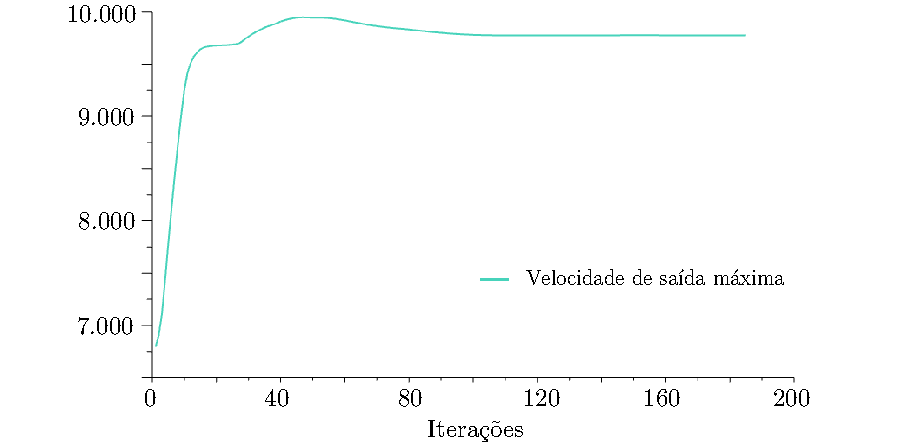
\includegraphics[width=0.90\textwidth]{Figuras/cfddecontinuidade2.pdf}  
    \caption{Convergência da velocidade de escoamento na saída do fluido do sistema.}  
    \legend{Fonte: o autor.}
    \label{fig:cfdcontinuidade2}  
\end{figure}

A convergência do modelo foi obtida com aproximadamente 180 iterações, conforme ilustra a Figura \ref{fig:cfdcontinuidade}. Embora seja possível visualizar uma
convergência a partir de 110 iterações para a velocidade média do escoamento na saída do sistema, como pode ser visualizado pelo gráfico da Figura \ref{fig:cfdcontinuidade2}. Assim, é possível inferir que houve convergência física do modelo durante todo o domínio físico, através da resolução de equações de fenômenos de transporte que caracterizam o escoamento de fluidos e validar a utilização do modelo de fluxo para obtenção do desgaste erosivo para este estudo. 

\section{Seleção dos atributos críticos}
\label{sec:Seleçãodosatributoscríticos} 

Antes de se realizar o planejamento de experimentos para obtenção da Superfície de reposta, é necessário um estudo prévio da influência dos atributos na função-objetivo de interesse. Para o caso em estudo, na análise de sensibilidade foram necessárias 15 simulações para realizar a variação de um atributo por vez, a partir do caso base em que as variáveis foram fixadas no nível intermediário (0). A Figura \ref{fig:efeitossensi} demonstra um gráfico do tipo tornado com os efeitos percentuais dos atributos na resposta de desgaste erosivo, o que permite observar se a mudança de nível (-1)
para (+1) de uma determinada variável resulta em aumento ou diminuição da taxa
erosiva, bem como os atributos que exercem maior impacto na resposta. 

\begin{figure}[H] 
    \centering  
    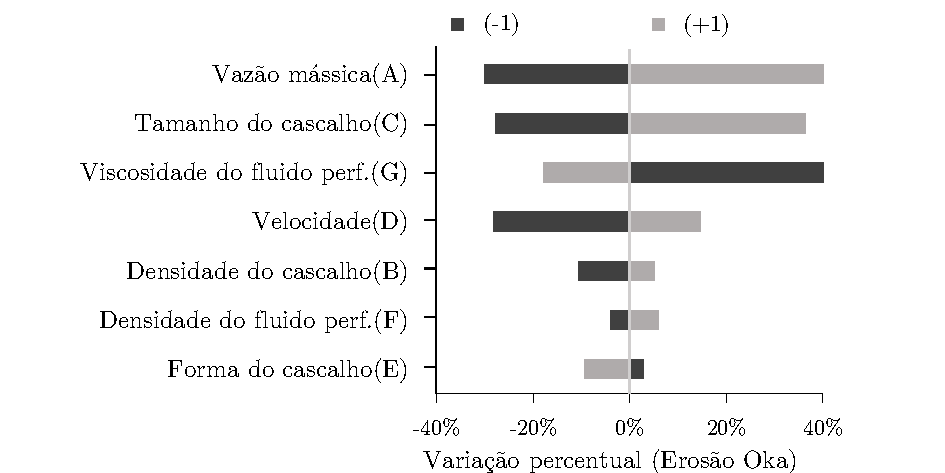
\includegraphics{Figuras/analisesensi.pdf}  
    \caption{Gráfico de efeitos percentuais dos atributos no desgaste erosivo.}  
    \legend{Fonte: o autor.}
    \label{fig:efeitossensi}  
\end{figure}

Os atributos incertos: "Forma do cascalho" e a "Viscosidade do fluido de perfuração", foram investigados em relação à taxa erosiva. Os valores desses atributos foram estudados em dois níveis, -1 e +1. Observou-se que o aumento dessas variáveis resultou em uma diminuição na taxa erosiva. Esses resultados físicos estão em concordância com estudos anteriores \cite{yabuki}, \cite{walker}, \cite{hutchings}. Dentro das faixas de estudo consideradas, foi observado que as variáveis de "Vazão mássica", "Tamanho do cascalho", "Velocidade", "Densidade do cascalho" e "Densidade do fluido de perfuração" apresentaram um aumento no desgaste erosivo ao serem incrementadas do nível (-1) para o nível (+1). Esses resultados estão em conformidade com os trabalhos anteriores \cite{clark}, \cite{albu},\cite{kowsari}, \cite{kumar}, \cite{hutchings}, \cite{ANUR}. É possível verificar, que os atributos que mais influenciam taxa erosiva dentro das faixas estudadas das variáveis aleatórias foram, respectivamente, "Vazão mássica", "Tamanho do cascalho", "Viscosidade do fluido de perfuração" e "Velocidade". A "densidade do cascalho" e do "Fluido de perfuração" e a "Forma dos cascalhos" exerceram pouco impacto na resposta de erosão comparados aos demais atributos para as faixas estudadas de variação.

O método do planejamento estatístico de Plackett Burmann foi empregado nesta etapa também com a finalidade de realizar uma triagem dos atributos que mais influenciam na taxa desgaste erosivo de Oka. Na Tabela \ref{tab:anovaplack} são apresentadas as análises dos efeitos em relação aos atributos puros, deste modo é possível definir quais variáveis têm maior impacto sobre a função-objetivo, que por sua vez, foi obtida através da seleção do ponto da tubulação em que o valor de desgaste é mais severo nos diversos cenários de fluxo simulados, conforme demonstrado na Figura \ref{fig:maiorerosao}. A Tabela \ref{tab:anovaplack} apresenta a Análise de variância com os resultados da análise estatística obtidos pelo Planejamento de Plackett Burmann, apresentando as Somas de quadrados (SQ), Graus de liberdade (GL), Médias quadráticas (MQ) e valores dos testes estatísticos F e p associados a cada fonte de variação do estudo de Desgaste Erosivo. Essas fontes de variação incluem os fatores de interesse, como diferentes tratamentos ou grupos experimentais computacionais, além de possíveis fatores de confusão ou erros.


\begin{table}[!h]
\caption{Análise de variância para o planejamento Plackett-Burman.}
\begin{tabular*}{\textwidth}{@{\extracolsep{\stretch{1}}}*{6}{c}@{}}
 \toprule
Fonte & GL & SQ Aj. & MQ Aj. & Valor F & Valor-P \\
  \midrule

   
        Modelo* & 7 & 2.10E-09 & 2.99E-10 & 19.20 & 0.006 \\ 
        Linear* & 7 & 2.10E-09 & 2.99E-10 & 19.20 & 0.006 \\ 
        Vazão mássica* & 1 & 7.50E-10 & 7.49E-10 & 47.97 & 0.002 \\ 
        Densidade do cascalho & 1 & 1.00E-11 & 5.40E-12 & 0.34 & 0.589 \\ 
        Tamanho* & 1 & 6.50E-10 & 6.51E-10 & 41.70 & 0.003 \\ 
        Velocidade* & 1 & 2.10E-10 & 2.11E-10 & 13.55 & 0.021 \\ 
        Forma & 1 & 2.00E-11 & 2.48E-11 & 1.59 & 0.276 \\ 
        Densidade do fluido de perfuração & 1 & 4.00E-11 & 4.28E-11 & 2.74 & 0.173 \\ 
        Viscosidade* & 1 & 4.10E-10 & 4.13E-10 & 26.48 & 0.007 \\ 
        Erro & 4 & 6.00E-11 & 1.56E-11 & ~ & ~ \\ \
        Total & 11 & 2.16E-09 \\ 

\bottomrule   
\end{tabular*}
\label{tab:anovaplack}
\subcaption{* Termos estatisticamente significativos com intervalo de 95\% de confiança.}
\legend {Fonte: o autor.}
\end{table*}
\end{table}

A partir da análise da tabela de ANOVA, foram obtidas informações para a interpretação dos resultados do estudo. A tabela permitiu identificar os atributos que apresentam uma diferença significativa entre os grupos ou tratamentos analisados, indicando os fatores independentes que possuem um efeito estatisticamente relevante na variável dependente. A partir da análise das medidas de variabilidade, como os quadrados médios e os valores F associados aos Graus de Liberdade, foi utilizado o teste estatístico de Fischer para determinar a significância estatística do modelo obtido (Figura \ref{fig:fischerplackett}).

\begin{figure}[H] 
    \centering  
    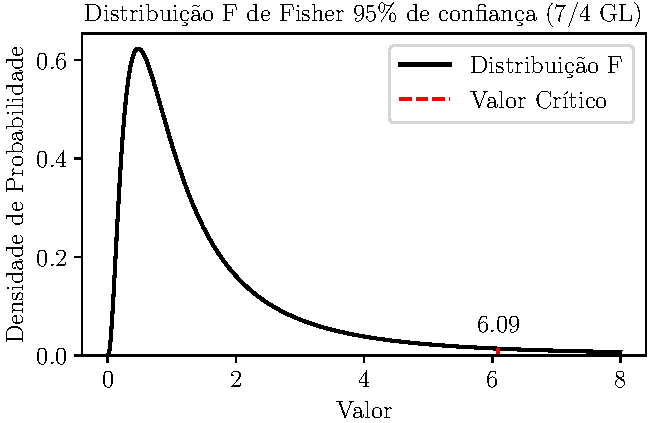
\includegraphics{Figuras/fischerplackett.pdf}  
    \caption{Distribuição de Fischer para análise de significância.}  
    \legend{Fonte: o autor.}
    \label{fig:fischerplackett}  
\end{figure}


A fonte de variação do "Modelo" refere-se ao modelo global utilizado na análise de variância. Conforme observado pela Figura \ref{fig:fischerplackett}, a distrubuição de Fischer para o modelo associado aos Graus de liberdade (7/4), indica um F crítico de 6.09 para um nível de significância de 95\%, o valor F calculado do modelo 19.20 indica que há uma diferença significativa entre os grupos ou tratamentos considerados neste estudo (com um valor-p associado de 0.006). Isso significa que as variáveis independentes têm um efeito estatisticamente relevante na variável dependente. Foram efetuados os cálculos de F para todos os termos com seus respectivos Graus de Liberdade o que determinou os Atributos com significância estatística. As variáveis: "Vazão mássica", "Tamanho do cascalho", "Velocidade" e "Viscosidade do fluido" apresentaram valores F significativos, indicando que elas têm um impacto estatisticamente significativo no Desgaste Erosivo.

A Figura \ref{fig:efeitosplackett} analisa os efeitos principais dos atributos em relação ao desgaste erosivo, o que permite observar se a mudança de nível (-1) para (+1) de uma determinada variável resulta em aumento ou diminuição da taxa erosiva. 





\begin{figure}[H] 
    \centering  
    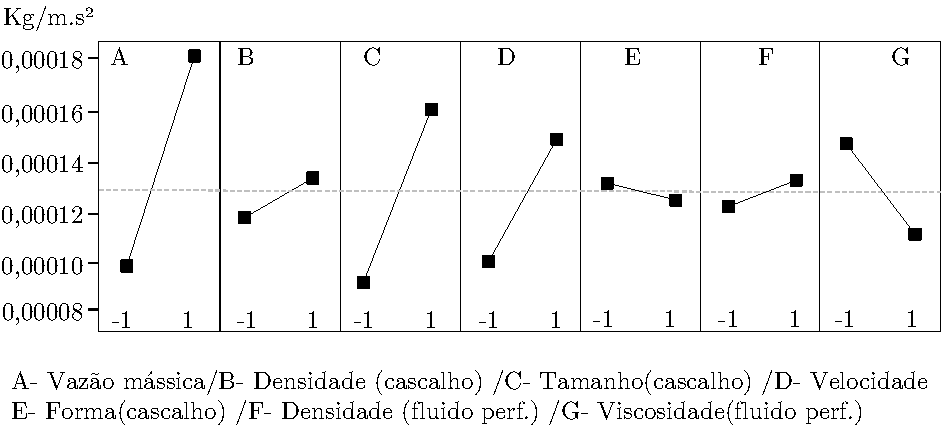
\includegraphics{Figuras/efeitosPLACKETT.pdf}  
    \caption{Gráfico de efeitos principais com médias ajustadas para o Desgaste erosivo.}  
    \legend{Fonte: o autor.}
    \label{fig:efeitosplackett}  
\end{figure}

Dentro das faixas de estudo consideradas, verificou-se que os atributos incertos "Forma" e "Viscosidade" apresentaram uma diminuição na taxa erosiva quando houve a mudança de nível de (-1) para (+1). Isso indica que o aumento dessas variáveis resulta em uma redução no desgaste erosivo. Por outro lado, observou-se que as variáveis "Vazão mássica", "Tamanho do cascalho", "Velocidade", "Densidade do cascalho" e "Densidade do fluido de perfuração" apresentaram um aumento no desgaste erosivo ao serem incrementadas do nível -1 para o nível +1. Esses resultados estão em conformidade com estudos anteriores que também relataram essas relações entre as variáveis e o Desgaste erosivo \cite{yabuki}, \cite{walker}, \cite{hutchings},\cite{clark}, \cite{albu},\cite{kowsari}, \cite{kumar}, \cite{hutchings}, \cite{ANUR}. A Figura \ref{fig:paretoplackett} apresenta o gráficos de Pareto dos efeitos principais para a resposta da taxa Desgaste erosivo de Oka. Este gráfico exibe de forma rápida e objetiva os efeitos que foram estatisticamente significativos com 95 \% de nível de significância, ou seja, os que apresentam valores resultantes maiores que a linha tracejada em vermelho.

\begin{figure}[H] 
    \centering  
    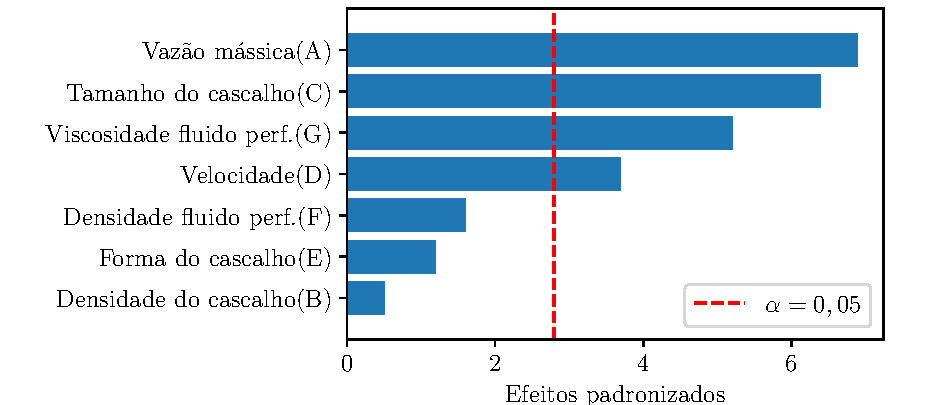
\includegraphics{Figuras/PLACKETTBURMANNNN.pdf}  
    \caption{Gráfico de pareto dos efeitos padronizados.}  
    \legend{Fonte: o autor.}
    \label{fig:paretoplackett}  
\end{figure}

Observando os resultados da Tabela \ref{tab:anovaplack} e Figura \ref{fig:paretoplackett}, os atributos "Forma do cascalho", "Densidade do fluido perfuração" e "Densidade do cascalho", não exerceram impacto significativo sobre o Desgaste erosivo, uma vez que seus respectivos valores F foram menores que os valores críticos para o intervalo de confiança de 95\%. Para validar as resposta do modelo gerado por Plackett Burmann foi necessária a realização de testes estatísticos recomendados por \citeonline{montgomery}. Para tanto, foram gerados os gráficos de probabilidade normal e análise de homocedasticidade dos resíduos (Figuras \ref{fig:probnormalplackett} e \ref{fig:residuosplackett}).

\begin{figure}[H] 
    \centering  
    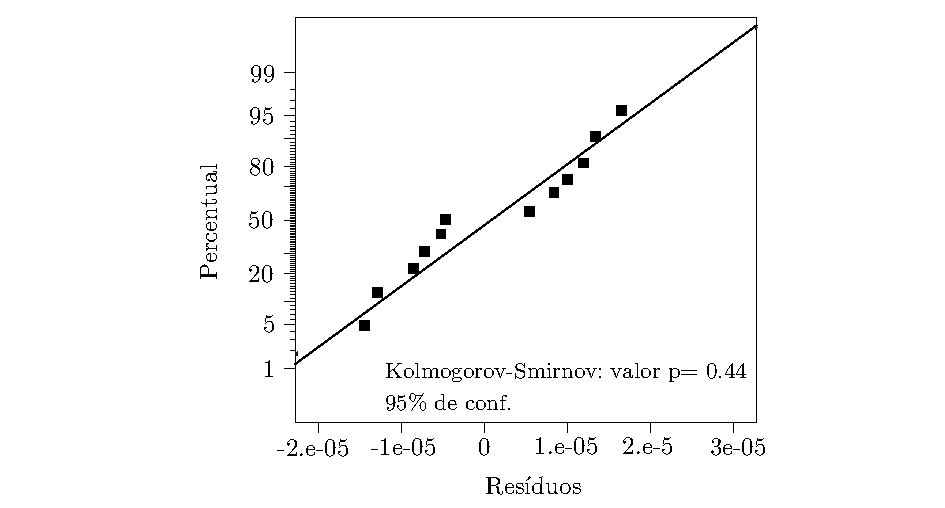
\includegraphics[width=0.92\textwidth]{Figuras/probnormalplacket.pdf}  
    \caption{Gráfico de probabilidade normal.}  
    \legend{Fonte: o autor.}
    \label{fig:probnormalplackett}  
\end{figure}


\begin{figure}[H] 
    \centering  
    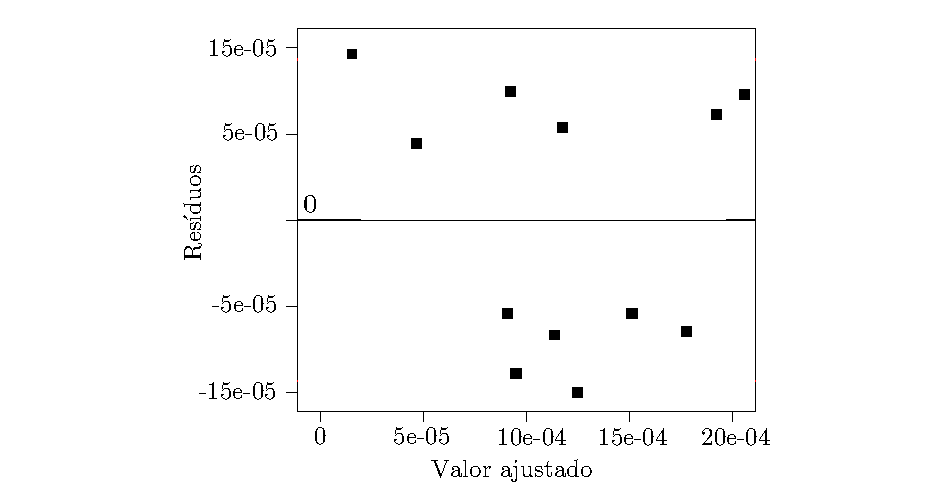
\includegraphics[width=0.92\textwidth]{Figuras/residuosPLACKETT.pdf}  
    \caption{Gráfico de resíduos versus Valores ajustados.}  
    \legend{Fonte: o autor.}
    \label{fig:residuosplackett}  
\end{figure}

Deste modo, através da análise das Figuras \ref{fig:probnormalplackett} e \ref{fig:residuosplackett} é possível verificar que os resíduos apresentam distribuição normal e homocedasticidade, ou seja, aleatoriedade em torno de um valor médio. Para validar esta hipótese, foi realizado o teste de normalidade de Kolmogorov-Smirnov. Para o ensaio de Plackett-Burmann realizado, o valor p do teste Kolmogorov-Smirnov foi de 0.44, o que indica que os resíduos seguem uma distribuição normal. Os métodos de Análise de sensibilidade e planejamento fatorial Plackett Burmann apresentaram respostas semelhantes em termos dos atributos críticos. Os parâmetros: "Vazão mássica", "Tamanho do cascalho", "Viscosidade fluido perfuração" e "Velocidade" evidenciaram significância estatística para a função-objetivo. Consequentemente, essas variáveis serão incorporadas na geração dos metamodelos de regressão por Superfície de Resposta e utilizadas na obtenção das curvas de risco. Por outro lado, os demais atributos foram mantidos no nível mais provável (0) em todas as etapas posteriores, resultando em uma redução no número de simulações numéricas necessárias nas etapas de Superfície de Resposta e Análise de Risco. Essa redução contribui para uma diminuição do tempo computacional necessário para realizar tais análises.


\section{Planejamento estatístico (Superfície de resposta)}

Na seção \ref{sec:Planejamentoestatistico}, o Planejamento fatorial fracionário Plackett Burmann foi utilizado para realizar a triagem dos atributos incertos de perfuração de poços, ou seja, para selecionar as variáveis mais significativas para o processo de Análise de risco. Nesta etapa, o planejamento de experimentos é aplicado para encontrar a Superfície de resposta, ou seja, a equação de regressão que irá compor o metamodelo para substituição das simulações computacionais no processo de Análise de risco. Os fatores estudados neste planejamento foram restringidos aos quatro identificados como significativos no planejamento de Plackett Burmann, sendo eles: "Vazão mássica(A)", "Tamanho do cascalho(C)", "Viscosidade fluido perf.(G)" e "Velocidade(D)". Deste modo, a matriz de planejamento criada foi composta por 25 pontos, sendo 1 ponto central, o que representa 25 modelos para serem simulados por fluidodinâmica computacional. De posse de todos os modelos simulados, foi realizada uma regressão multivariada, e foram obtidos os termos da Superfície de Resposta estatísticamente significativos através da Análise de Variância (Tabela \ref{tab:anovabox}).

\begin{table}[!h]
\caption{Análise de variância do modelo de regressão (Superfície de resposta).}
\begin{tabular*}{\textwidth}{@{\extracolsep{\stretch{1}}}*{6}{c}@{}}
 \toprule
  Fonte&SQ (Aj.)&	GL	&QM (Aj.)&	Valor F& Valor P\\
  \midrule

Modelo(Regressão)*&	1.87E-09&	8&	2.34E-10&	53.91&	< 0.0001\\
Vazão mássica*&	6.59E-10&	1&	6.59E-10&	151.85&	< 0.0001\\
Viscosidade*&	1.81E-10&	1&	1.81E-10&	41.68&	< 0.0001\\
Tamanho*&	6.32E-10&	1&	6.32E-10&	145.44&	< 0.0001\\
Velocidade*&3.07E-10&	1&	3.07E-10&	70.72&	< 0.0001\\
Vazão mássica x Viscosidade* &	1.52E-11&	1&	1.52E-08&	3.50&	0.0497\\
Tamanho x Velocidade*&	1.98E-11&	1&	1.98E-08&	4.56	&0.0485\\
Vazão mássica²*&	2.25E-11&	1&	2.25E-11&	5.18&	0.0370\\
Tamanho²*&	5.05E-11&	1&	5.05E-11&	11.64&	0.0036\\
Resíduo&	6.95E-11&	16	&4.34E-12	\\	
Total&	1.94E-09&	24	\\		

  \bottomrule   
\end{tabular*}
\label{tab:anovabox}
\subcaption{* Termos estatisticamente significativos com intervalo de 95\% de confiança.}
\legend {Fonte: o autor.}
\end{table*}
\end{table}

A tabela de Análise de Variância foi empregada para examinar os resultados do estudo e identificar os atributos que demonstram diferenças estatisticamente significativas entre os grupos ou tratamentos analisados. Essa análise possibilitou determinar quais fatores independentes apresentam um efeito estatisticamente relevante na variável dependente, por se tratar de um estudo de Superfície de Resposta através do planejamento estatístico de Box Behnkhen, é possível verificar além dos termos lineares, os termos de interação e quadráticos. Para isso, foram consideradas medidas de variabilidade, como os quadrados médios e os valores F associados aos Graus de Liberdade. O teste estatístico de Fischer foi utilizado para verificar a significância estatística do modelo obtido. Essa abordagem permitiu uma interpretação dos resultados, destacando os fatores que exercem influência estatisticamente relevante no desgaste erosivo.


\begin{figure}[H] 
    \centering  
    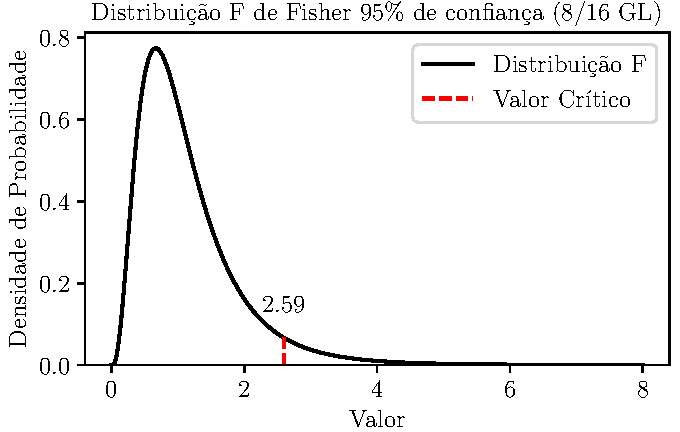
\includegraphics{Figuras/fischerbox.pdf}  
    \caption{Distribuição de Fischer para análise de significância.}  
    \legend{Fonte: o autor.}
    \label{fig:fischerbox}  
\end{figure}


Através da análise de Figura \ref{fig:fischerbox}, é possível verificar que o Modelo de Regressão gerado a partir do planejamento de Box Benhkhen é válido estatisticamente. O valor de F calculado (53.91) do modelo, levando em consideração o número de graus de liberdade do planejamento, é superior ao F crítico (2.59) para 95\% de nível de significância. Foram efetuados os cálculos
de F para todos os termos com seus respectivos Graus de Liberdade o que determinou os atributos com significância estatística para o modelo. A partir da validação estatística do modelo de regressão incluindo os termos lineares, quadráticos e de interação significativos, foi possível gerar a equação com os coeficientes dos termos para a previsão do desgaste de Erosão de Oka, que constitui o metamodelo (Equação \ref{eq:metamodelo}). 
 

\begin{equation}
\begin{align*} 
E = -5.4435x10^{-5} + 0.0003(A) + 1.6880x10^{-7}(G) - 0.0508(C) + 1.7630x10^{-6}(D)\\ 
- 2.7877x10^{-6}(A)(G) + 0.0114(C)(D) - 0.0004(A)^2 - 30.8644(C)^2 \quad \quad \quad \;  \, \, \, \, \, \, \,\, \\ 
\end{align*}
\label{eq:metamodelo}
\end{equation}

Onde:

E = é a taxa de erosão (kg/m.s²);

A= Vazão mássica (kg/s);

C= Tamanho do cascalho(mm);

D= Velocidade (m/s);

G= Viscosidade do fluido perf (cP). 
\vspace{1.2cm}



A partir da obtenção da equação de regressão, é possível a realização de previsões de taxa de Erosão. Para verificar a consistência dos resultados do modelo de regressão em relação aos resultados de simulação fluidodinâmica, foi realizada uma validação cruzada dos resultados de erosão obtidos pela simulação numérica e pelo metamodelo (Figura \ref{fig:validcruzada}). Estes cenários simulados e preditos foram obtidos através da combinação dos parâmetros utilizadas para gerar os metamodelos e suas respectivas respostas de taxa de Erosão. 

\begin{figure}[H] 
    \centering  
    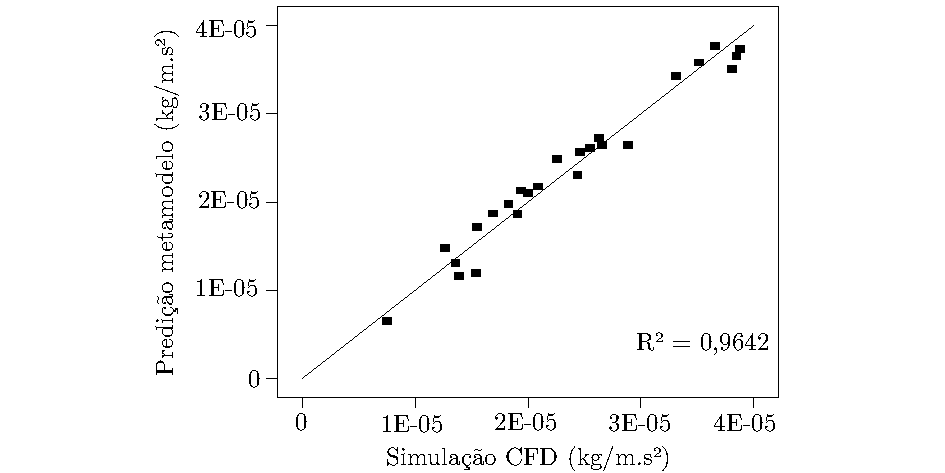
\includegraphics{Figuras/crossplotbehkhen.pdf}  
    \caption{Validação cruzada entre o modelo de Regressão e a simulação numérica CFD.}  
    \legend{Fonte: o autor.}
    \label{fig:validcruzada}  
\end{figure}

Por meio da análise da Figura \ref{fig:validcruzada}, é possível observar que o metamodelo está bem ajustado para as previsões de taxa de erosão, o que é esperado uma vez que os dados previstos foram os mesmos utilizados para geração do modelo. A presente análise constitui um procedimento preliminar, visando avaliar a adequação do modelo aos dados. É importante ressaltar que, em etapas subsequentes do estudo, serão realizados testes para verificar a capacidade de generalização do modelo para dados adicionais. Nesta etapa de avaliação do modelo, foi analisado o coeficiente de determinação R²=0.9642, o qual fornece um indicativo relevante sobre a capacidade preditiva do modelo. No entanto, é importante ressaltar que o valor de R² não oferece informações sobre possíveis vieses do modelo ou sua capacidade de generalização para dados não observados. Portanto, para mitigar esse aspecto, foi calculado o R² ajustado, uma métrica que considera a inclusão de variáveis adicionais no modelo e indica se elas contribuem significativamente para a capacidade de previsão. Além disso, foi obtido o R² previsto, uma medida de validação cruzada que avalia o desempenho do modelo ao remover sistematicamente cada observação da matriz de dados e estimar o valor correspondente com base na equação de regressão. Essa abordagem permite uma avaliação mais precisa da capacidade do modelo em lidar com dados não vistos anteriormente. A medida de Precisão adequada mede a relação sinal-ruído, que compara a faixa dos valores previstos nos pontos das observações com o erro médio de previsão, portanto razões maiores que 4 indicam  que o modelo é adequado. A Tabela \ref{tab:r2} demonstra o valores de R² e a Precisão adequada do modelo.


\begin{table}[!h]
\centering
\caption{Estatísticas de ajuste do modelo de regressão (Superfície de resposta).}
\begin{tabular*}{0.6\textwidth}{@{\extracolsep{\stretch{1}}}*{2}{c}@{}}
 \toprule
  Fonte&Valor\\
  \midrule

R²             & 0.9643  \\
R² Ajustado    & 0.9465  \\
R² Predito   & 0.9123  \\
Precisão adequada & 24.9635\\
Desvio padrão &2.08e-06\\
  \bottomrule   
\end{tabular*}
\label{tab:r2}

\legend {Fonte: o autor.}
\end{table*}
\end{table}

Os valores obtidos para  R², R² Predito e R² Ajustado, encontram-se muito próximos, considerando a pequena disparidade entre os valores em questão. Portanto a partir desta análise é possível inferir, através desta análise prévia, que não há razões para suspeitar que o modelo esteja viesado, o que será verificado de fato com a verificação da capacidade de generalização do modelo em dados ainda não vistos.

A medida de precisão adequada de 24.964 indica que o modelo possui uma proporção maior que 4 entre sinal e ruído. Isso sugere que a variação explicada pelos fatores independentes incluídos no modelo é significativamente maior do que a variação não explicada ou atribuível ao ruído aleatório.

Para serem utilizadas em previsões, o modelo deve atender a certos requisitos estatísticos \cite{montgomery}. Para tanto, foi aplicado o teste de normalidade (Figura \ref{fig:testeprobnormal}) para verificar se a distribuição dos resíduos aparenta ser normal.  Outra análise importante é a de que os resíduos devem possuir variância constante (homocedasticidade), ou seja, que o modelo de regressão obtido comete erros aleatórios e não prevê sistematicamente nenhum intervalo de valores de destino, a Figura \ref{fig:residuoshomoedasticidade} demonstra os resíduos do modelo.


\begin{figure}[H] 
    \centering  
    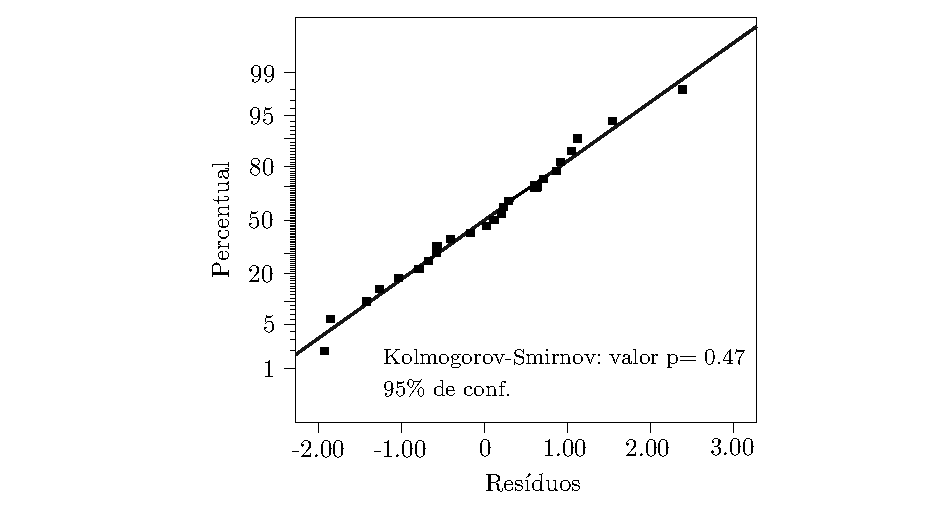
\includegraphics{Figuras/probnormal.pdf}  
    \caption{Gráfico de probabilidade normal.}  
    \legend{Fonte: o autor.}
    \label{fig:testeprobnormal}  
\end{figure}

\begin{figure}[H] 
    \centering  
    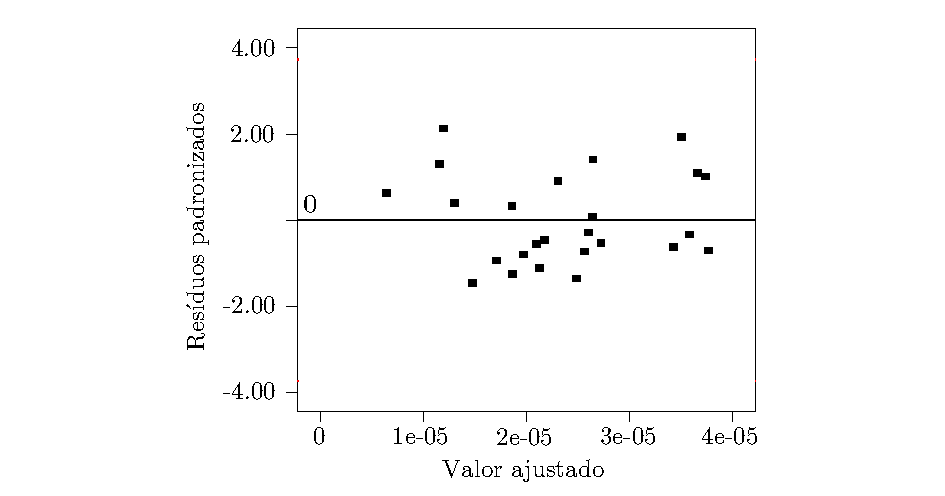
\includegraphics{Figuras/residuos.pdf}  
    \caption{Gráfico de resíduos padronizados.}  
    \legend{Fonte: o autor.}
    \label{fig:residuoshomoedasticidade}  
\end{figure}

A análise da Figura \ref{fig:testeprobnormal} permite determinar que os pontos se encontram próximos da linha reta, ou seja, a distribuição de erro é aproximadamente normal. Para validar esta hipótese, foi realizado o teste de normalidade de Kolmogorov-Smirnov. Para o ensaio de Box Behnken realizado, o valor p do teste Kolmogorov-Smirnov foi de 0.47, o que indica que os resíduos seguem uma distribuição normal. A Figura \ref{fig:residuoshomoedasticidade} não demonstra razão para suspeitar de qualquer violação das suposições de independência ou variância constante, ou seja, é possível verificar que os resíduos apresentam homocedasticidade.
Esse modelo de regressão gerado é composto por uma equação analítica, que contém termos lineares, quadráticos e de interação, que foram considerados como significativos através da análise de variância (Tabela \ref{tab:anovabox}). Na Tabela \ref{tab:box555} encontram-se os valores de erosão simulados para elaboração da superfície de resposta e os valores previstos pelo metamodelo de regressão, a partir das mesmas combinações dos parâmetros.

\begin{table}[H]
\caption{Matriz do planejamento Box Benhkhen para 4 variáveis de entrada.}
\begin{tabular*}{\textwidth}{@{\extracolsep{\stretch{1}}}*{7}{c}@{}}
 \toprule
   Simulação &VM	&VISC	&TAM	&VEL&Erosão OKA&Erosão Modelo	\\
  \midrule

1  & 0.13 & 15 & 0.55  & 9.50  & 1,92E-05 & 1,86E-05 \\
2  & 0.27 & 15& 0.55  & 9.50   & 3,88E-05 & 3,73E-05 \\
3  & 0.13 & 35& 0.55  & 9.50   & 1,28E-05 & 1,47E-05 \\
4  & 0.27 & 35 & 0.55  & 9.50  & 2,47E-05 & 2,57E-05 \\
5  & 0.20  & 25  & 0.24 & 8.87  & 1,36E-05 & 1,30E-05 \\
6  & 0.20  & 25  & 0.86 & 8.87  & 2,44E-05 & 2,31E-05 \\
7  & 0.20  & 25  & 0.24 & 10.13 & 1,70E-05 & 1,87E-05 \\
8  & 0.20  & 25  & 0.86 & 10.13 & 3,66E-05  & 3,76E-05 \\
9  & 0.13 & 25  & 0.55  & 8.87  & 1,38E-05 & 1,16E-05 \\
10 & 0.27 & 25  & 0.55  & 8.87  & 2,66E-05 & 2,64E-05 \\
11 & 0.13 & 25  & 0.55  & 10.13 & 2,09E-05 & 2,17E-05 \\
12 & 0.27 & 25  & 0.55  & 10.13 & 3,85E-05 & 3,66E-05 \\
13 & 0.20  & 15 & 0.24 & 9.50   & 1,83E-05 & 1,97E-05 \\
14 & 0.20  & 35 & 0.24 & 9.50   & 1,54E-05 & 1,20E-05 \\
15 & 0.20  & 15 & 0.86 & 9.50   & 3,31E-05 & 3,42E-05 \\
16 & 0.20  & 35 & 0.86 & 9.50   & 2,88E-05 & 2,65E-05 \\
17 & 0.13 & 25 & 0.24& 9.50  & 7,55E-06 & 6,46E-06 \\
18 & 0.27 & 25  & 0.24 & 9.50   & 1,95E-05 & 2,13E-05 \\
19 & 0.13 & 25  & 0.86 & 9.50   & 2,00E-05 & 2,10E-05 \\
20 & 0.27 & 25  & 0.86 & 9.50   & 3,51E-05 & 3,58E-05 \\
21 & 0.20  & 15 & 0.55  & 8.87  & 2,26E-05 & 2,49E-05 \\
22 & 0.20  & 35 & 0.55  & 8.87   & 1,56E-05 & 1,71E-05 \\
23 & 0.20  & 15 & 0.55  & 10.13 & 3,80E-05 & 3,50E-05 \\
24 & 0.20  & 35 & 0.55  & 10.13 & 2,63E-05 & 2,72E-05 \\
25 & 0.20  & 25  & 0.55  & 9.5    & 2,56E-05 & 2,61E-05\\

\bottomrule 
\end{tabular*}
\label{tab:box555}
\subcaption{VM: Vazão massica(kg/s); VISC: Viscosidade do fluido de perfuração(cP); TAM: Tamanho(mm); VEL: Velocidade de escoamento(m/s).}
\legend {Fonte: o autor.}
\end{table}


Após a validação estatística do modelo de Box Behnkhen, foram gerados as figuras com os termos lineares, quadráticos e de interação que compõe o modelo. Estes gráficos visam demonstrar como os termos influenciam na resposta do modelo. A Figura \ref{fig:efeitosbox1} 
apresenta o Gráfico de efeitos dos termos lineares que compõe o modelo. 


\begin{figure}[H] 
    \centering  
    \includegraphics{Figuras/efeitosdeinteracao - Cópia.pdf}  
    \caption{Gráfico de efeitos para o desgaste erosivo de Oka.}  
    \legend{Fonte: o autor.}
    \label{fig:efeitosbox1}  
\end{figure}

É possível observar que a Vazão mássica, Tamanho e Velocidade apresentam efeitos positivos no desgaste erosivo, ou seja, o aumento desses atributos ocasionam maiores desgates dentro das respectivas faixas de variação. O atributo Velocidade causa um aumento linear na resposta de erosão, enquanto que os atributos de Vazão mássica e Tamanho não apresentam relação linear com a variação do nível do atributo. 

Avaliar efeitos de interações é um dos principais objetivos dos planejamentos estatísticos. Se uma interação entre diferentes atributos for significativa, indica que a resposta de um fator depende da presença ou ausência do outro para a modelagem. Para estes casos, é pertinente o estudo do comportamento de um fator em relação a cada nível de outro fator. Em muitos casos, como o analisado na Tabela \ref{tab:anovabox}, somente alguns termos de interações contribuem efetivamente para a Soma de Quadrados da Interação e com significância adequadas para constituir o metamodelo de regressão.  As interações entre os atributos "Vazão mássica" e Viscosidade e "Tamanho e Velocidade", consideradas como significativas para o modelo, através da Análise de variância da Tabela \ref{tab:anovabox} se encontram dispostas na Figura \ref{fig:efeitosdeint}.

\begin{figure}[H] 
    \centering  
    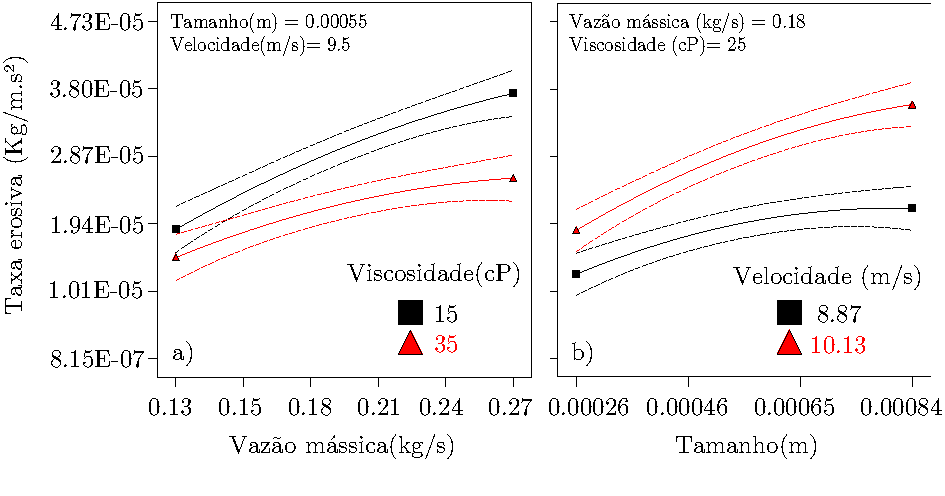
\includegraphics[width=0.95\textwidth]{Figuras/efeitosdeinteracao.pdf}  
    \caption{Efeitos de interação dos termos significativos do modelo de Box Behnken.}  
    \legend{Fonte: o autor.}
    \label{fig:efeitosdeint}  
\end{figure}



Através da análise da Figura \ref{fig:efeitosdeint}(a), é possível observar a interação entre "Vazão mássica e Viscosidade", o aumento da "Vazão mássica" propicia um desgaste erosivo maior em um nível inferior de "Viscosidade", e em "Viscosidade" mais alta embora haja um aumento da taxa erosiva, a magnitude de desgaste não é tão elevado quanto em menor "Viscosidade". Na Figura \ref{fig:efeitosdeint}(b) através da interação entre "Velocidade e Tamanho", é possível observar que numa condição de "Velocidade" maior e concomitante aumento de "Tamanho", dentro da faixa estudada, a taxa erosiva é mais elevada. Enquanto em "Velocidade" mais baixa, embora haja um aumento da taxa erosiva, a magnitude de desgaste não é tão elevado quanto em maior "Velocidade". A Figura \ref{fig:respostaveltam2o}, demonstra os gráficos de Superfície de resposta e contorno decorrente da interação dos atributos de "Viscosidade e Vazão mássica". Estes gráficos fornecem uma clara inspeção visual das interações entre os atributos e a magnitude na função-objetivo de desgaste erosivo.

\begin{figure}[H] 
    \centering  
    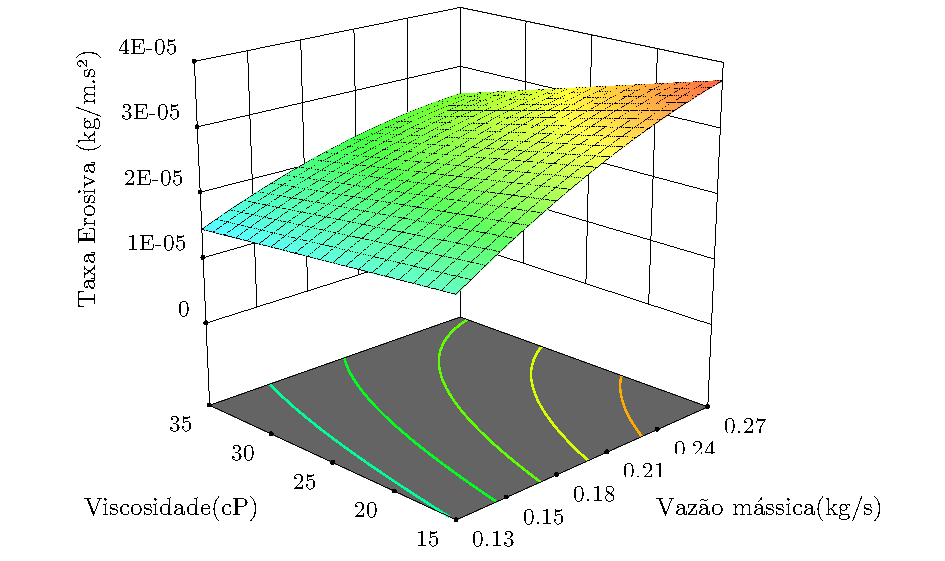
\includegraphics[width=0.88\textwidth]{Figuras/superficie2.pdf}  
    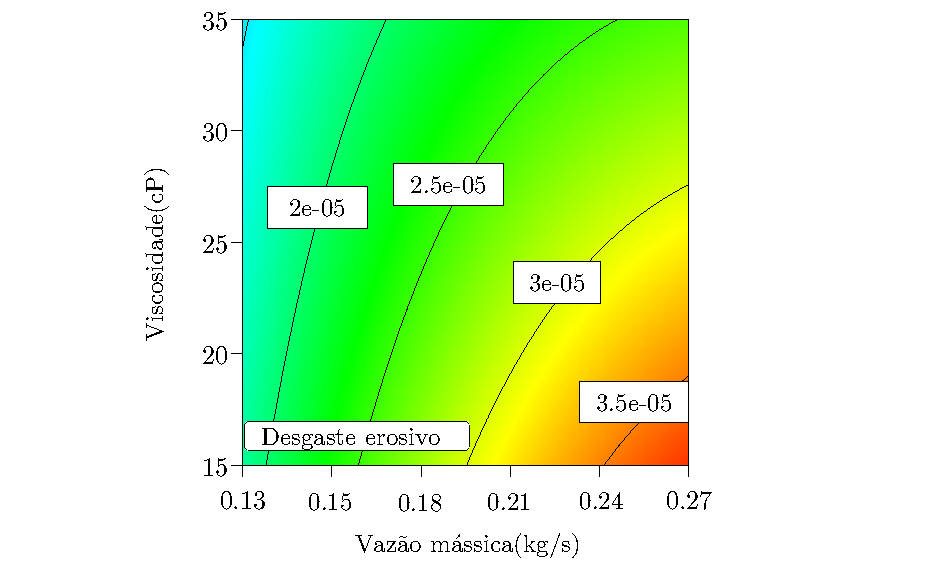
\includegraphics[width=0.88\textwidth]{Figuras/contornomassica.pdf}  
    \caption{Superfície de resposta e gráfico de contorno do efeito de Velocidade e Tamanho na resposta de taxa erosiva.}  
    \legend{Fonte: o autor.}
    \label{fig:respostaveltam2o}  
\end{figure}

Na análise da Figura \ref{fig:respostaveltam2o}, é evideciada a interação entre os termos de "Viscosidade do fluido de perfuração e Vazão mássica". Observa-se que a "Viscosidade" exerce uma influência direta na resposta da taxa erosiva. Para valores menores de "Viscosidade", é observada uma maior magnitude da taxa erosiva. Isso ocorre porque, nessas condições, as partículas sólidas têm maior tendência a se depositar na superfície do material, resultando em colisões mais frequentes nas paredes do material. Do contrário, uma maior "Viscosidade de fluido" causa uma maior tendência das partículas seguirem as linhas de corrente, o que reduz a frequência de impacto e, consequentemente, a taxa erosiva \cite{tsai}, \cite{yabuki}. A maior concentração de partículas presentes no fluxo, ou seja, aumento de "Vazão mássica" resulta em maior propensão ao desgaste, haja vista que a Erosão aumenta com a quantidade de partículas incidindo sobre a superfície do material alvo \cite{gandhi}. Assim, conforme o modelo, o aumento concomitante da "Viscosidade e Vazão mássica", provém o incremento da taxa erosiva para as faixas de variação estudadas. A Figura \ref{fig:respostaveltama}, demonstra os gráficos de Superfície de resposta e contorno decorrente da interação dos atributos de "Velocidade e Tamanho do cascalho".

\begin{figure}[H] 
    \centering  
    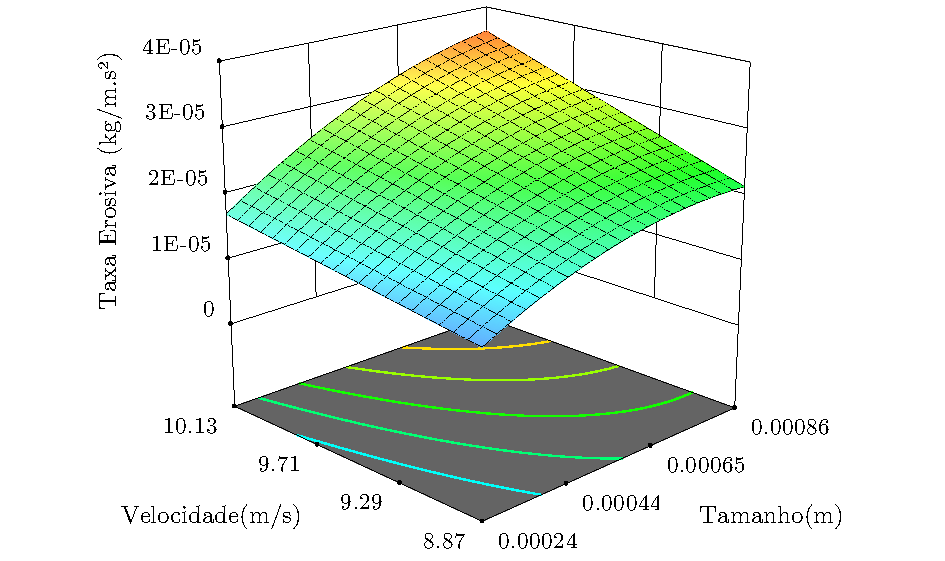
\includegraphics[width=0.84\textwidth]{Figuras/superficie.pdf}  
    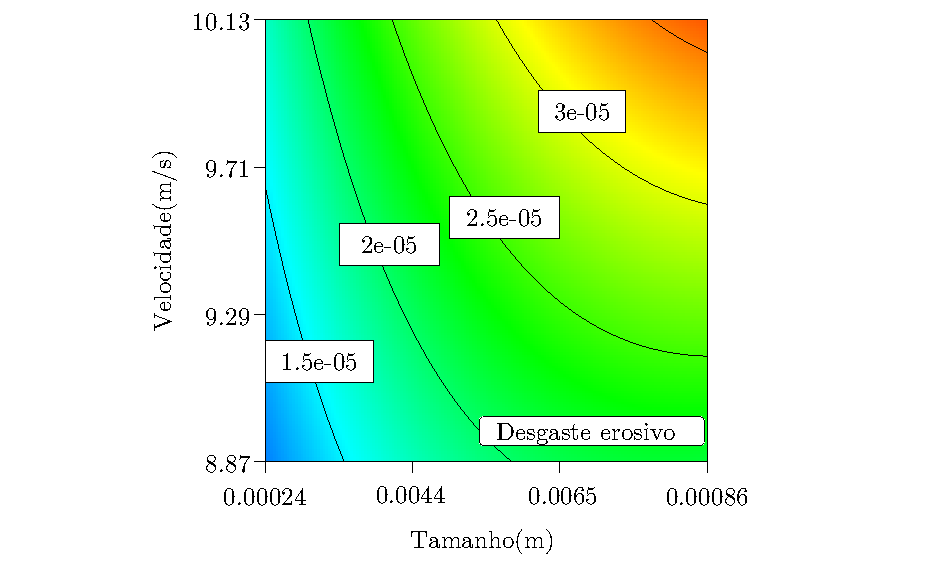
\includegraphics[width=0.84\textwidth]{Figuras/contorno2.pdf} 
    \caption{Superfície de resposta do efeito de Velocidade e Tamanho na resposta de taxa erosiva.}  
    \legend{Fonte: o autor.}
    \label{fig:respostaveltama}  
\end{figure}

Através da Figura \ref{fig:respostaveltama} é possível observar que partículas maiores resultam no aumento da taxa de erosão. Isto é explicado pois, além da maior energia de impacto, o tamanho da superfície de contato entre a partícula e a superfície tende a ser mais abrangente, levando a um maior desgaste no material \cite{lieb}, \cite{clark}. De mesmo modo, é possível verificar que em maiores Velocidades ocorre o aumento da taxa erosiva, em função da maior energia cinética de impacto \cite{lind}, \cite{finnie2}. De acordo com o metamodelo matemático, foi observada que o aumento concomitante dos valores dos atributos "Vazão mássica" e "Velocidade" resulta em cenários com maior desgaste erosivo, dentro das faixas de variação consideradas no estudo. Isso indica que os parâmetros influenciam de forma conjunta na resposta do modelo, e o aumento de seus valores contribui para um aumento no desgaste erosivo.

\section{Análise de risco através da Árvore de derivação}

Neste item, são obtidas e comparadas as curvas de Árvore de derivação por simulação numérica CFD e o modelo de regressão obtido pelo metamodelo de Superfície de resposta. O método da Árvore de derivação resultou em 81 cenários de simulação numérica, através da combinação de 3 níveis para as 4 variáveis definidas como críticas para o desgaste erosivo na etapa de triagem. Após simulação fludidinâmica dos cenários determinados, os dados foram tratados estatisticamente para obtenção da curva de risco de falha por Desgaste Erosivo (Figura \ref{fig:ad}).


\begin{figure}[H] 
    \centering  
    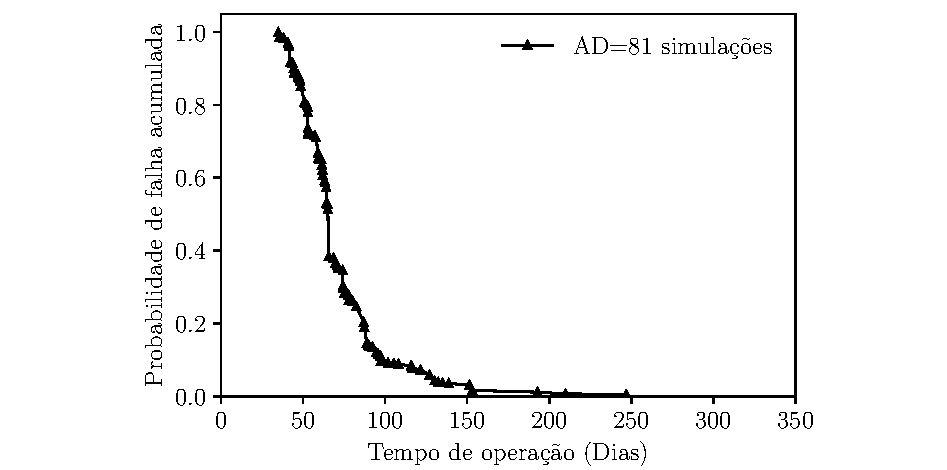
\includegraphics{Figuras/AD.pdf}  
    \caption{Árvore de derivação para 4 atributos com 3 níveis.}  
    \legend{Fonte: o autor.}
    \label{fig:ad}  
\end{figure}

Através da análise da curva de risco, é possível observar que os valores correspondentes aos percentis desse processo são respectivamente, P10 = 97.40 dias, P50 = 64.91 dias e P90 = 44.21 dias. As Figura \ref{fig:scattermodelo} e \ref{fig:compmetaarvore}, exibem os gráficos de validação cruzada e os valores comparativos entre os valores obtidos pelo metamodelo de regressão e as 81 simulações fluidodinâmicas CFD que compuseram a Árvore de derivação.

\begin{figure}[H] 
    \centering  
    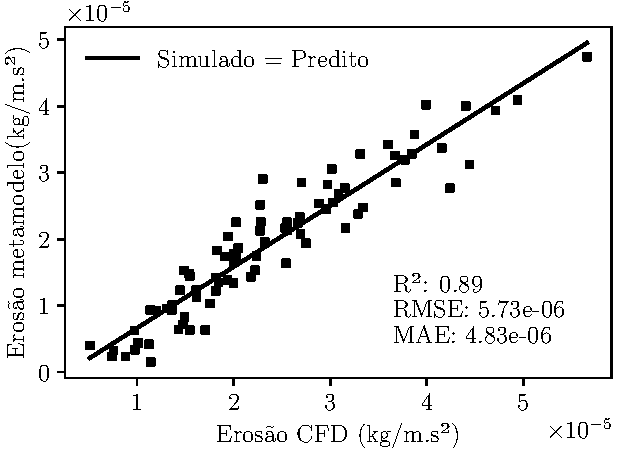
\includegraphics{Figuras/scatterModelo2.pdf}  
    \caption{Validação cruzada entre o metamodelo de Regressão e a simulação numérica CFD.}  
    \legend{Fonte: o autor.}
    \label{fig:scattermodelo}  
\end{figure}
\begin{figure}[H] 
    \centering  
    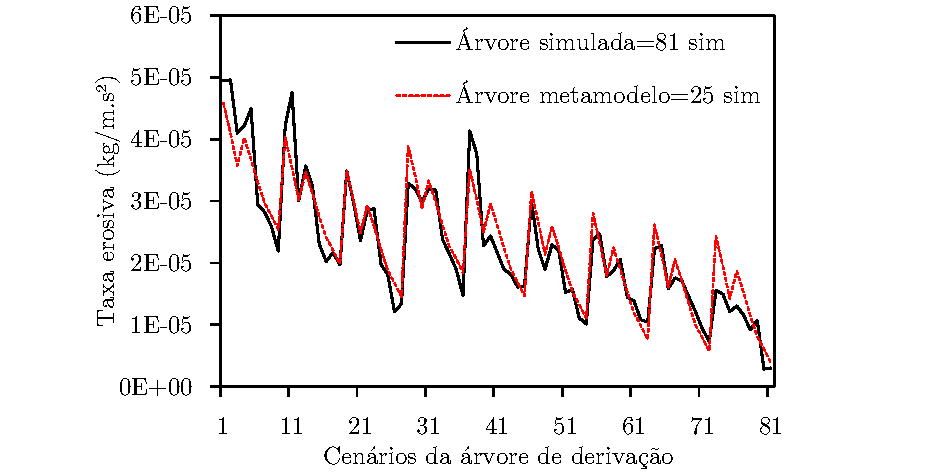
\includegraphics{Figuras/compmetaarvore.pdf}  
    \caption{Comparativo (Erosão CFD e Erosão pelo metamodelo de regressão.}  
    \legend{Fonte: o autor.}
    \label{fig:compmetaarvore}  
\end{figure}


Os resultados obtidos com o metamodelo de regressão demonstram uma capacidade satisfatória de prever os cenários da Árvore de derivação, como evidenciado pelas métricas R², RMSE e MAE. Isso indica que o modelo possui capacidade de realizar previsões em dados que não foram utilizados para a constituição do modelo. A Figura \ref{fig:compmetaarvore} ilustra como o modelo se ajustou adequadamente às variações das respostas dos cenários simulados pela Árvore de derivação. Além disso, a Figura \ref{fig:AdeAD} apresenta a comparação entre a curva de risco de falha por Erosão obtida por Simulações fluidodinâmicas computacionais para o método da Árvore de derivação e a curva de Árvore de derivação prevista pelo metamodelo de regressão.

\begin{figure}[H] 
    \centering  
    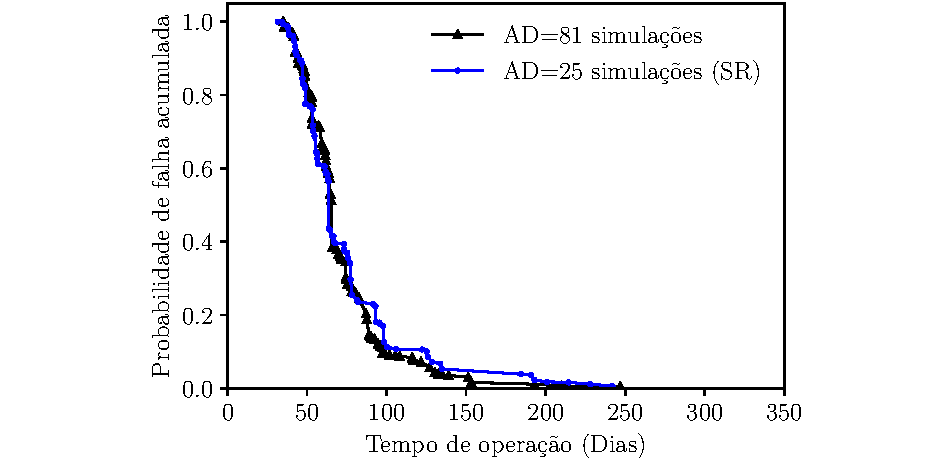
\includegraphics{Figuras/probacADeSR.pdf}  
    \caption{Curvas de risco por Árvore de derivação (CFD e Metamodelo).}  
    \legend{Fonte: o autor.}
    \label{fig:AdeAD}  
\end{figure}


Ao analisar o gráfico, podemos constatar que a curva de risco gerada pelo modelo de regressão se ajustou de forma satisfatória e apresentou uma proximidade significativa em relação à curva de referência, a qual é composta por todos os pontos simulados por CFD, assim como nos resultados de trabalhos anteriores para Análise de risco para estudos econômicos de projetos petrolíferos \cite{loschiavo},\cite{steagall}, \cite{santoss2}, \cite{yeten}, \cite{risso1}, \cite{slotte}  . Isso indica que o metamodelo é capaz de fornecer uma estimativa adequada da curva de risco. Para a curva de Árvore de derivação obtida pelo metamodelo foram necessárias 25 simulações fluidodinâmicas, o que representa uma redução de aproximadamente 69\% do número de simulações requeridas para obtenção da curva de risco, resultando em um esforço computacional menor. A Tabela \ref{tab:percentisadsr} apresenta a comparação dos percentis (P10, P50 e P90) entre a curva de risco obtida pela simulação numérica e pela superfície de resposta.

\begin{table}[h]
\caption{Comparação entre os percentis das curvas de risco de falha por simulação CFD e Metamodelo (SR).}
\begin{tabular*}{\textwidth}{@{\extracolsep{\stretch{1}}}*{4}{c}@{}}
 
  \toprule
    Percentil& Árvore de derivação (CFD) & Árvore de derivação (SR)  & Variação  \\
  (\%)& falha (dias) & falha (dias) &(\%)   \\
  \midrule
   P10&	97.40 	&100.70 &3.27\%\\
  P50 &	 64.91	&63.64& -1.95\%\\
 P90 &	44.21	&45.16 &2.14\%\\

  \bottomrule   
\end{tabular*}
\label{tab:percentisadsr}
\legend {Fonte: o autor.}
\end{table*}
\end{table}

A curva obtidas pelo modelo de regressão aplicada à árvore de derivação demonstrou bons resultados sendo o maior diferencial de percentis de 3.27\% para o P10, -1.95\% para o P50 e 2.14\% para o P90, comparado com a curva de Árvore de derivação simulada de referência. O próximo capítulo demonstra as curvas de risco pelo método de Monte Carlo obtidas pelo metamodelo de regressão.

\section{Análise de risco através de Monte Carlo}

     Nesta etapa, foi realizada a geração das curvas de risco segundo os sorteios de Monte Carlo e comparadas com a Árvore de derivação gerada por simulações fluidodinâmicas. Para a composição das curvas de risco por Monte Carlo foram obtidos diferentes cenários variando entre 100 e 80000 valores, seguindo a distribuição de probabilidade das variáveis aleatórias. Os resultados de erosão de cada cenário realizado pelos sorteios foram obtidos pelo metamodelo de regressão. Com as amostras obtidas por Monte Carlo, é possível a obtenção da média e desvio padrão da erosão para cada distribuição amostral, e deste modo realizar o cálculo de Cov (coeficiente de variação) para cada conjunto (Figura \ref{fig:mc}).  


\begin{figure}[H] 
    \centering  
    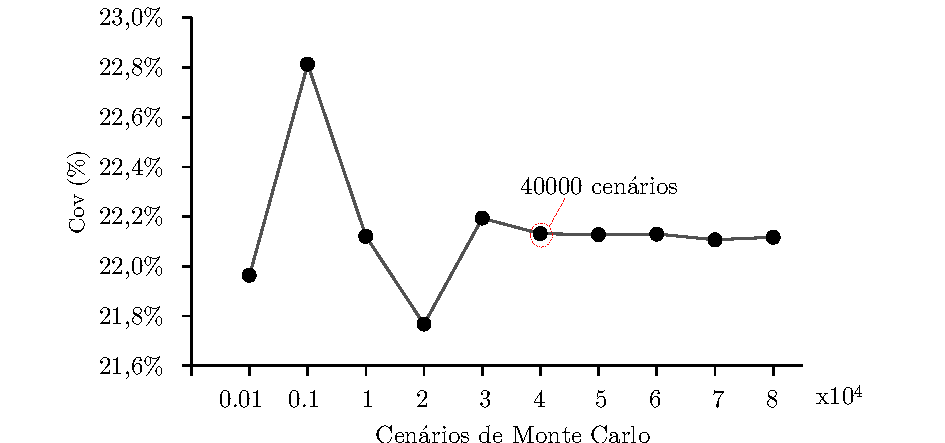
\includegraphics[width=0.83\textwidth]{Figuras/mcsorteios.pdf}  
    \caption{Coeficiente de variação para os cenários de Monte Carlo.}  
    \legend{Fonte: o autor.}
    \label{fig:mc}  
\end{figure}

 É possível verificar através da análise do Cov, que a partir de 40000 amostras, a erosão do modelo de Oka passa a produzir uma estimativa consistente da função de distribuição de probabilidade. A Figura \ref{fig:mca} demonstra as distribuições de probabilidade de diferentes quantidades amostrais obtidas por Monte Carlo.

\begin{figure}[H] 
    \begin{minipage}[!]{0.50\linewidth}
    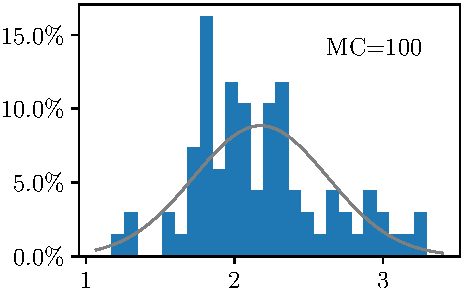
\includegraphics[\width=\linewidth]{Figuras/100.pdf}
    \end{minipage}
    \begin{minipage}[!]{0.50\linewidth}
    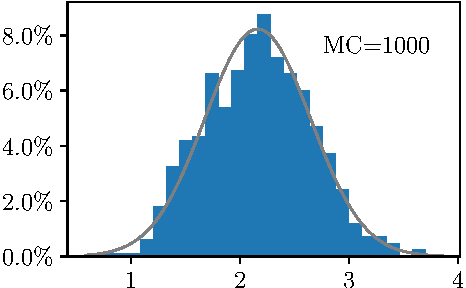
\includegraphics[\width=\linewidth]{Figuras/1000.pdf}
    \end{minipage}
    \begin{minipage}[!]{0.50\linewidth}
    \centering
    \includegraphics[\width=\linewidth]{marca}\\ {Erosão kg/m.s² (x10^{-5})}
    \end{minipage}
    \begin{minipage}[!]{0.50\linewidth}
    \centering
    \includegraphics[\width=\linewidth]{marca}\\ {Erosão kg/m.s² (x10^{-5})}
    \end{minipage}
   

    \begin{minipage}[!]{0.50\linewidth}
    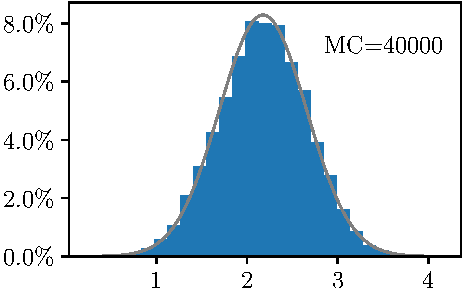
\includegraphics[\width=\linewidth]{Figuras/40000.pdf}
    \end{minipage}
    \begin{minipage}[!]{0.50\linewidth}
    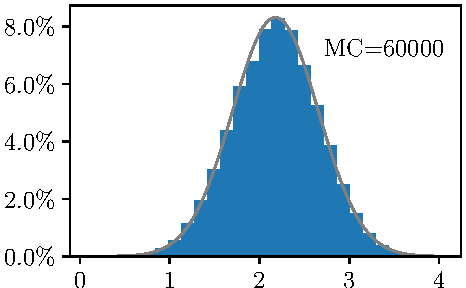
\includegraphics[\width=\linewidth]{Figuras/60000.pdf}
    \end{minipage}
    \begin{minipage}[!]{0.50\linewidth}
    \centering
    \includegraphics[\width=\linewidth]{marca}\\ {Erosão kg/m.s² (x10^{-5})}
    \end{minipage}
    \begin{minipage}[!]{0.50\linewidth}
    \centering
    \includegraphics[\width=\linewidth]{marca}\\ {Erosão kg/m.s² (x10^{-5})}
    \end{minipage}
    \caption{Distribuição da resposta de Erosão em diferentes cenários de Monte Carlo.}
    \legend{Fonte: o autor.}
    \label{fig:mca}
\end{figure}

Através das distribuições de probabilidade, é verificado que em 100 cenários de Monte carlo a curva de distribuição ainda não apresenta uma estimativa consistente da distribuição da resposta, conforme aumenta o número de cenários é possível constatar que a média e desvio-padrão se estabilizam e a curva apresenta distribuição estável e consistente. A Figura \ref{fig:mc222} demonstra as comparações das distribuições segundo as diferentes combinações de cenários de Monte Carlo, o que reforça o indicativo de estabilização a partir de 40.000 cenários de combinações das variáveis para geração da resposta. 


\begin{figure}[H] 
    \centering  
    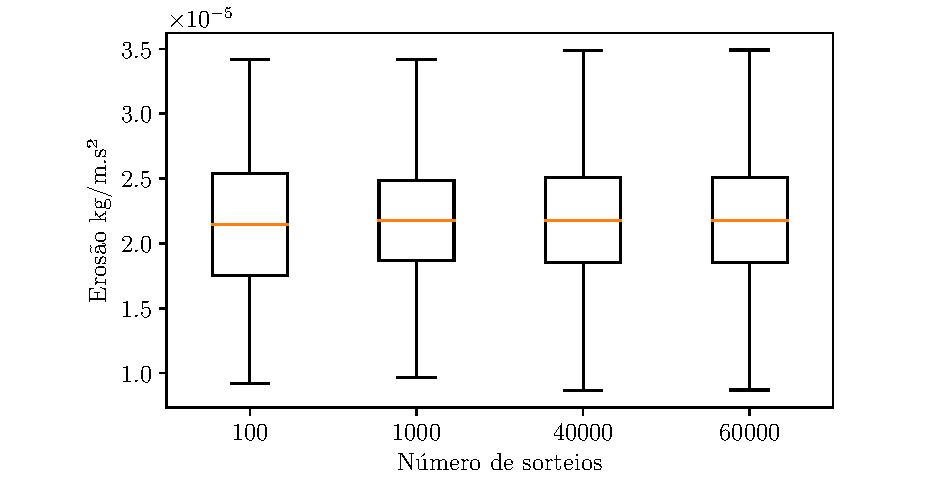
\includegraphics{Figuras/boxplots.pdf}  
    \caption{Box plots da Distribuição da resposta de Erosão em diferentes cenários de Monte Carlo.}  
    \legend{Fonte: o autor.}
    \label{fig:mc222}  
\end{figure}

A partir das respostas obtidas foram plotadas curvas de risco geradas pelos diferentes cenários
de sorteios, para avaliar a influência na qualidade da curva de risco. A Figura \ref{fig:mc2} apresenta a curva de risco de falha por erosão, obtidas por Árvore de derivação (CFD) e as obtidas pelos cenários gerados por Monte Carlo.


\begin{figure}[H] 
    \centering  
    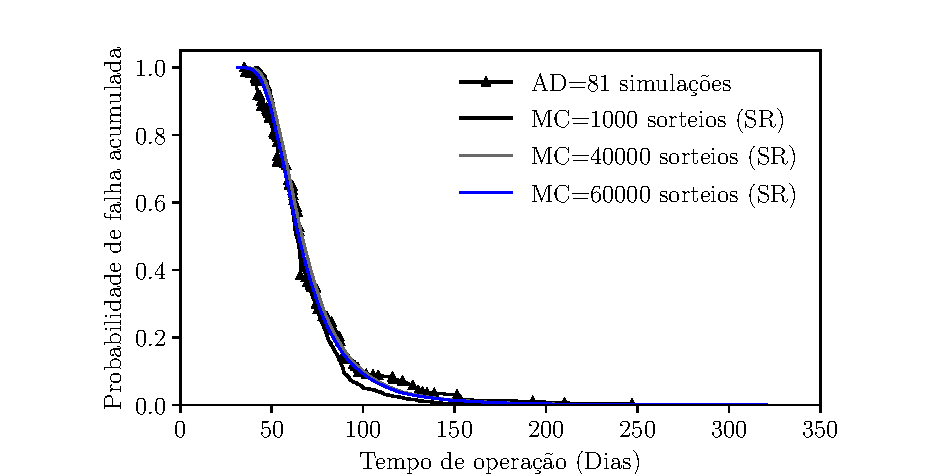
\includegraphics{Figuras/mc.pdf}  
    \caption{Curvas de risco Monte Carlo e Árvore de derivação.}  
    \legend{Fonte: o autor.}
    \label{fig:mc2}  
\end{figure}



Os sorteios gerados pelo método de Monte Carlo com as distribuições das variáveis contínuas, e com a aplicação da superfície de resposta, apresentaram curvas muito próximas da obtida pela Árvore de derivação gerada com 81 simulações fluidodinâmicas, especialmente as curvas com 40000 sorteios e 60000 sorteios. Como não houve grande variação entre os sorteios de 40000 e 60000 é aceitável determinar que 40000 cenários evidencia o número de sorteios ideal para reprodução da distribuição dos atributos para previsão do desgaste erosivo. A Tabela \ref{tab:percentisadmc} apresenta a comparação dos percentis (P10, P50 e P90) entre a curva de risco da Árvore de derivação, obtida pela simulação numérica e as curvas de Monte Carlo geradas pelo modelo de superfície de resposta.


\begin{table}[h]
\caption{Comparação entre os percentis das curvas de risco de falha por simulação CFD e Metamodelo (SR) para cenários de Monte Carlo.}
\begin{tabular*}{\textwidth}{@{\extracolsep{\stretch{1}}}*{5}{c}@{}}
 
  \toprule
    Percentil&  MC 1000 (SR) & MC 40000 (SR)& MC 60000 (SR)&MC 80000(SR)  \\
 (\%) &   Variação(\%) &Variação(\%)& Variação(\%)& Variação(\%)  \\
  \midrule
   P10	& 8.41\%&1,45\%&1.43\%&1.52\%\\
  P50 	& 0.47\%&0.62\%& 0.59\%&0.61\%\\
 P90 	& 16.03\%&1.99\%&2.08\%&2.11\%\\

  \bottomrule   
\end{tabular*}
\label{tab:percentisadmc}
\subcaption{Diferenças percentuais em módulo.}
\legend {Fonte: o autor.}

\end{table*}
\end{table}

A curva de risco obtida através da técnica de Monte Carlo com 1000 sorteios apresenta diferença de 16.03\% em relação ao percentil P90, 8.41\% em relação ao P10 e 0.47\% para P50 da curva gerada por Simulação computacional para Árvore de derivação. Porém, as curvas de risco geradas com 40000, 60000 e 80000 sorteios de Monte Carlo se encontram muito próximas entre si e em relação à curva de risco de Árvore de derivação de referência.  Deste modo, é possível verificar que as variações percentuais atingiram estabilização, não havendo grandes mudanças nas magnitudes dos percentis com o aumento de sorteios a partir de 40000 combinações de Monte Carlo, o que reitera as análises gráficas das Figuras \ref{fig:mc}, \ref{fig:mca} e \ref{fig:mc222}.

As diferenças percentuais entre os valores obtidos para os percentis da Árvore de derivação e Monte Carlo, ocorre pelas diferenciações que as técnicas apresentam quanto ao método de combinação dos atributos aleatórios para geração dos cenários de erosão. Neste sentido, o método de Monte Carlo apresenta maior confiabilidade do ponto de vista amostral, uma vez que as são obtidas quantidades amostrais sificientemente representativas para composição das simulações até que se alcance estabilidade numérica na resposta. Por outro lado, os cenários obtidos através do método de Árvore de derivação gerados a partir da discretização dos atributos, embora seja mais simples do ponto de vista amostral, obteve os resultados de desgaste erosivo diretamente a partir de simulações numéricas por CFD, não sendo necessário obrigatoriamente uma aplicação de um modelo de regressão para previsão dos dados de resposta.

Ademais, as obtenções dos desgastes erosivos de \citeonline{oka} para o método de Monte Carlo, foram obtidas pelo metamodelo de regressão, o que apresenta erros de aproximação inerentes aos métodos de regressão. Estes resultados demostram que a técnica de Monte Carlo e a técnica de Árvore de derivação apresentam resultados similares para obtenção de curva de risco de falha por erosão, uma vez que sejam utilizados metamodelos validados estatísticamente e sorteios amostrais suficientemente representativos das distribuições das variáveis aleatórias. Sendo métodos que podem ser aplicados concomitantemente para uma análise de risco mais rigorosa e com maior confiabilidade para a tomada de decisão referente à projetos do setor petrolífero.

  




